\chapter{Presentation of finished work}

In this section I will present and showcase my finished appliction. I will include screenshots to have a better representation and understanding for the reader.
The camera function in the application allows you to capture the current state of the graphs, which in this case came in handy for documentation.


\begin{figure}[!ht]
    \centering
    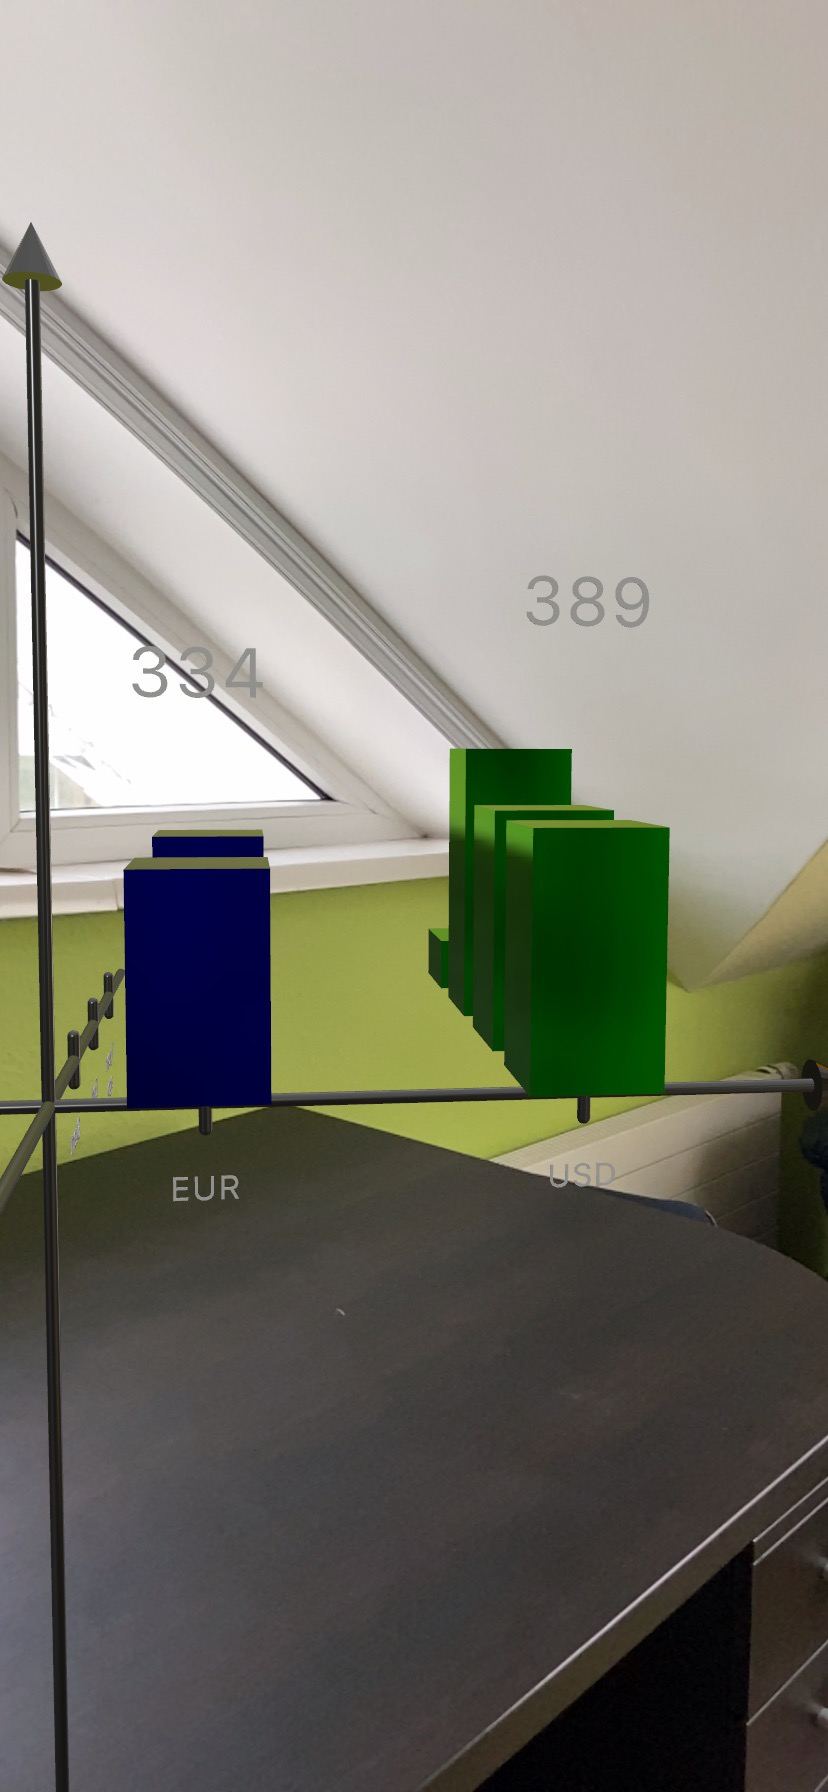
\includegraphics[scale=0.2]{../images/front.jpeg}
    % \includegraphics[width=150mm, keepaspectratio]{figures/TeXnicCenter.png}
    \caption{The main screen of the application.}
    \label{fig:TexnicCenter}
\end{figure}

\begin{figure}[!ht]
    \centering
    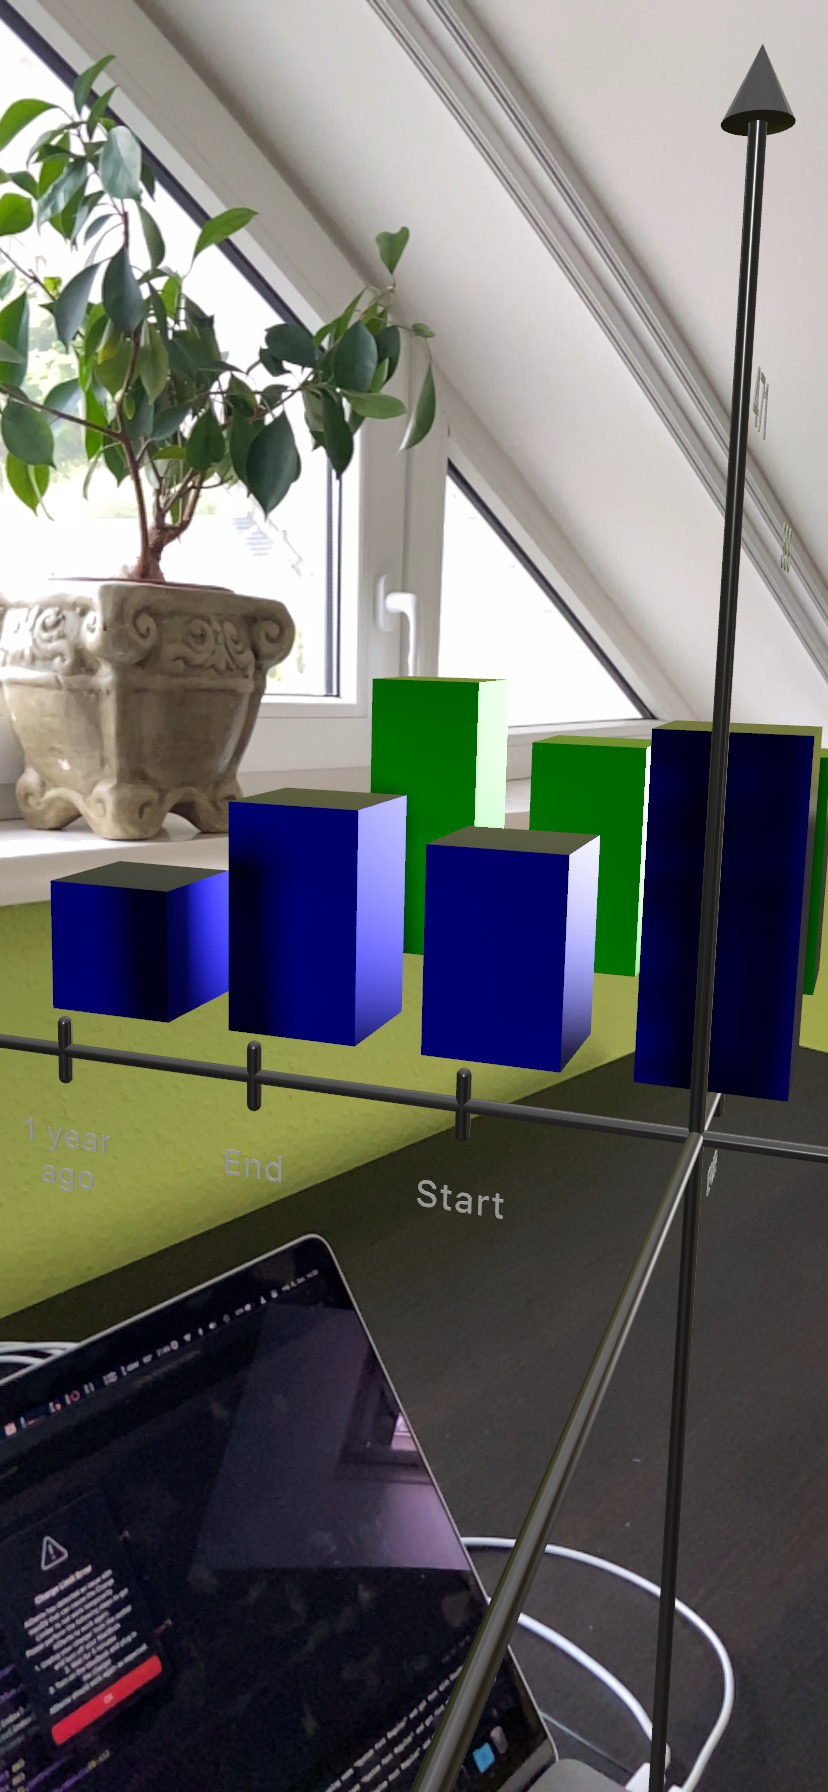
\includegraphics[scale=0.2]{../images/side.jpeg}
    % \includegraphics[width=150mm, keepaspectratio]{figures/TeXnicCenter.png}
    \caption{The main screen of the application.}
    \label{fig:TexnicCenter}
\end{figure}

\begin{figure}[!ht]
    \centering
    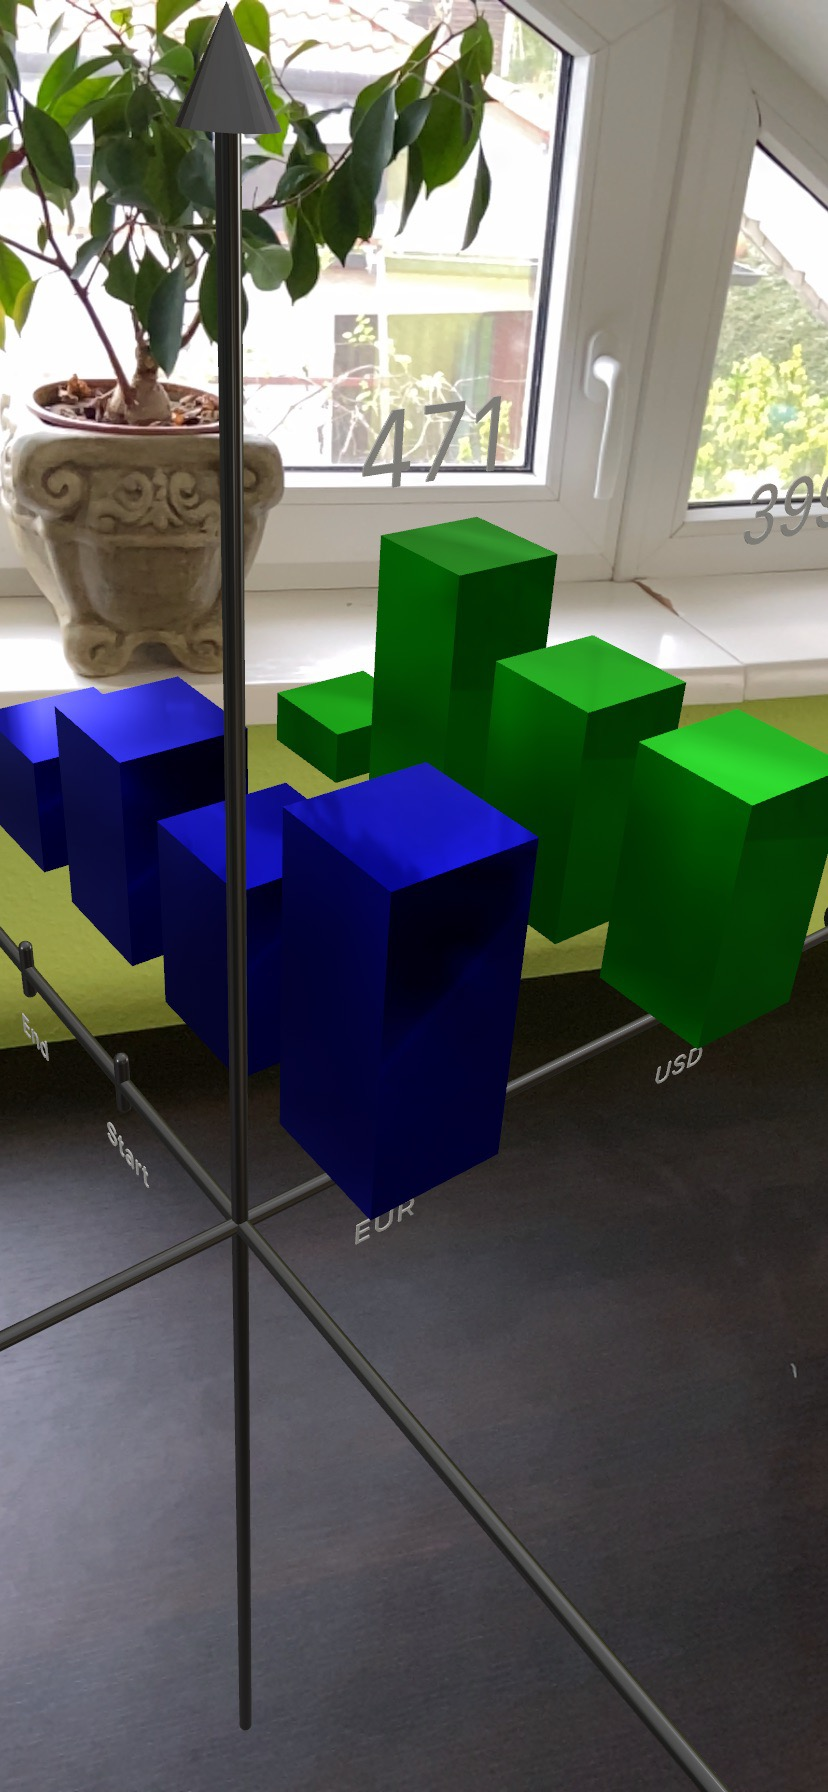
\includegraphics[scale=0.2]{../images/top.jpeg}
    % \includegraphics[width=150mm, keepaspectratio]{figures/TeXnicCenter.png}
    \caption{The main screen of the application.}
    \label{fig:TexnicCenter}
\end{figure}

As the attached images clearly show, the virtual 3D graph can be easily walked around and viewed from different angles, thereby giving users a new comparative perspective. It is possible to move and rotate the entire graph, as well as move the current exchange rate columns to make it easier to compare with other metrics. The move and rotate functions are only available in Spectate mode, for this you have to stop Live mode (or otherwise start Live mode) by pressing the button located in the upper left corner.

Currently, 2 currencies are available in the application, but of course this can be easily expanded at any time in the future. These two are EUR to HUF and USD to HUF. These can be displayed after selection and confirmation from the bottom bar. If the given exchange rate is already placed, it can no longer be added to the graph twice.

\begin{figure}[!ht]
    \centering
    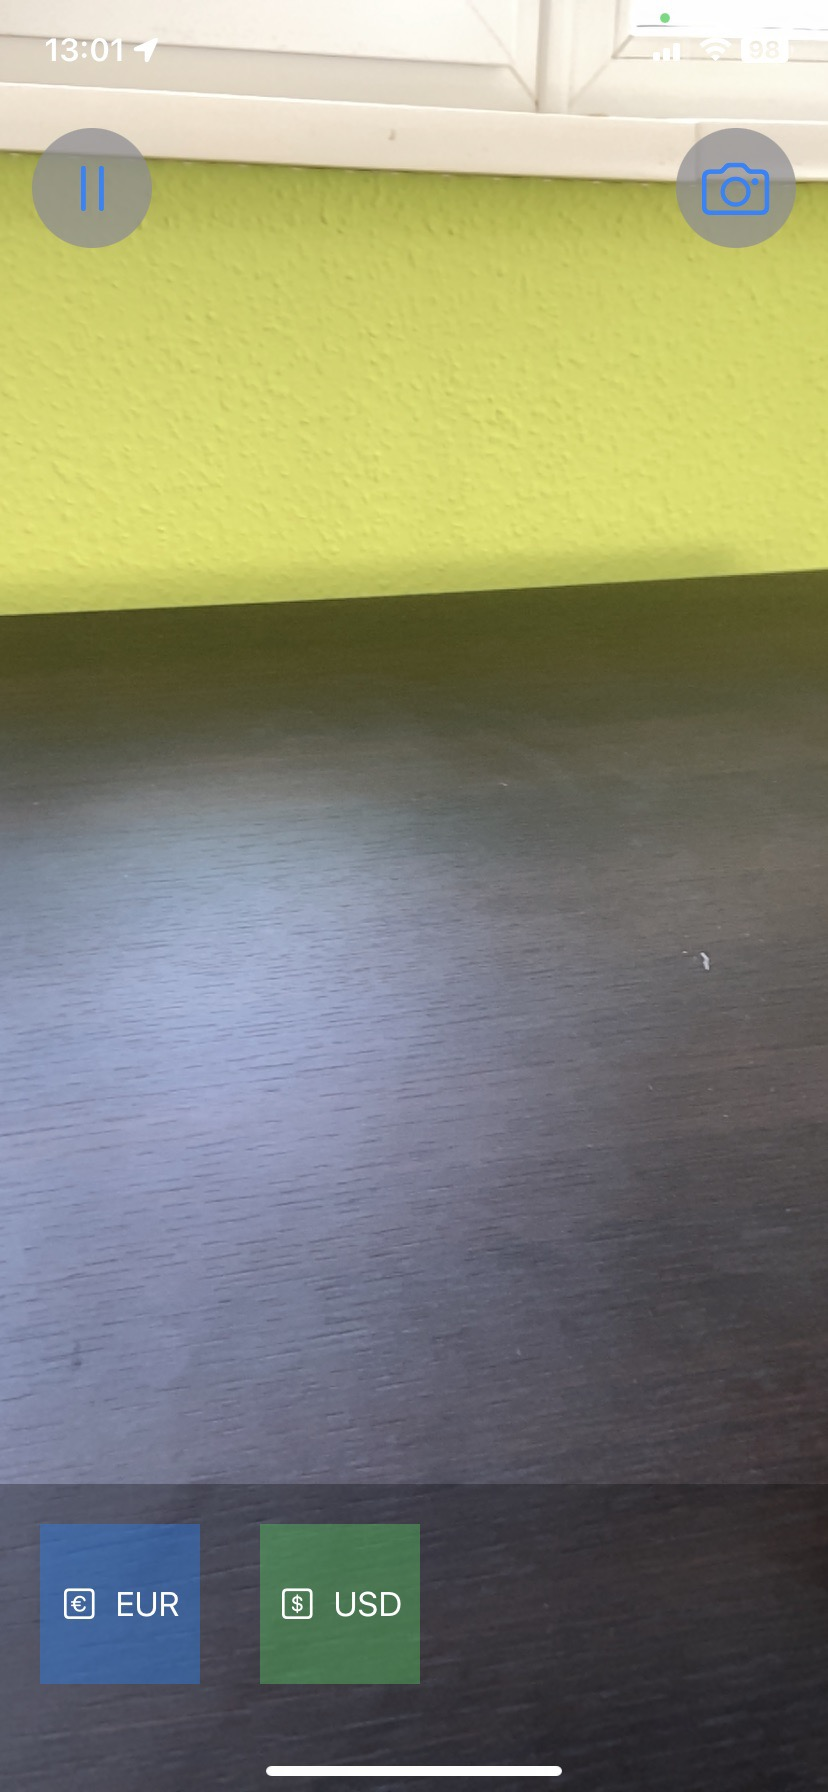
\includegraphics[scale=0.2]{../images/selector.jpeg}
    % \includegraphics[width=150mm, keepaspectratio]{figures/TeXnicCenter.png}
    \caption{The main screen of the application.}
    \label{fig:TexnicCenter}
\end{figure}

\begin{figure}[!ht]
    \centering
    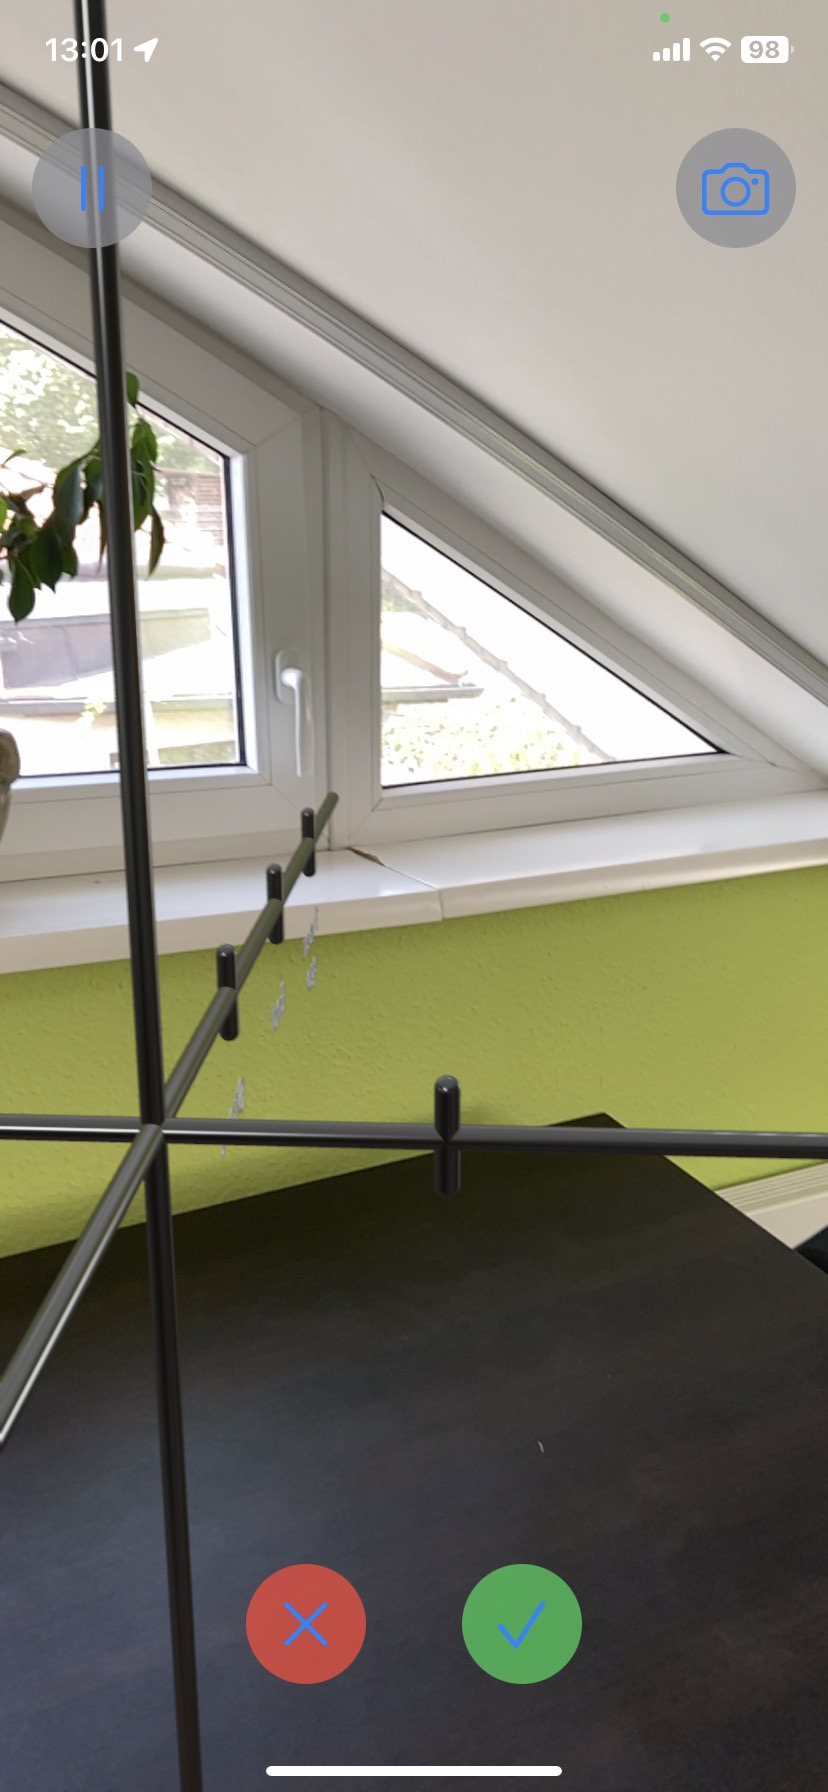
\includegraphics[scale=0.2]{../images/megerosites.jpeg}
    % \includegraphics[width=150mm, keepaspectratio]{figures/TeXnicCenter.png}
    \caption{The main screen of the application.}
    \label{fig:TexnicCenter}
\end{figure}

\begin{figure}[!ht]
    \centering
    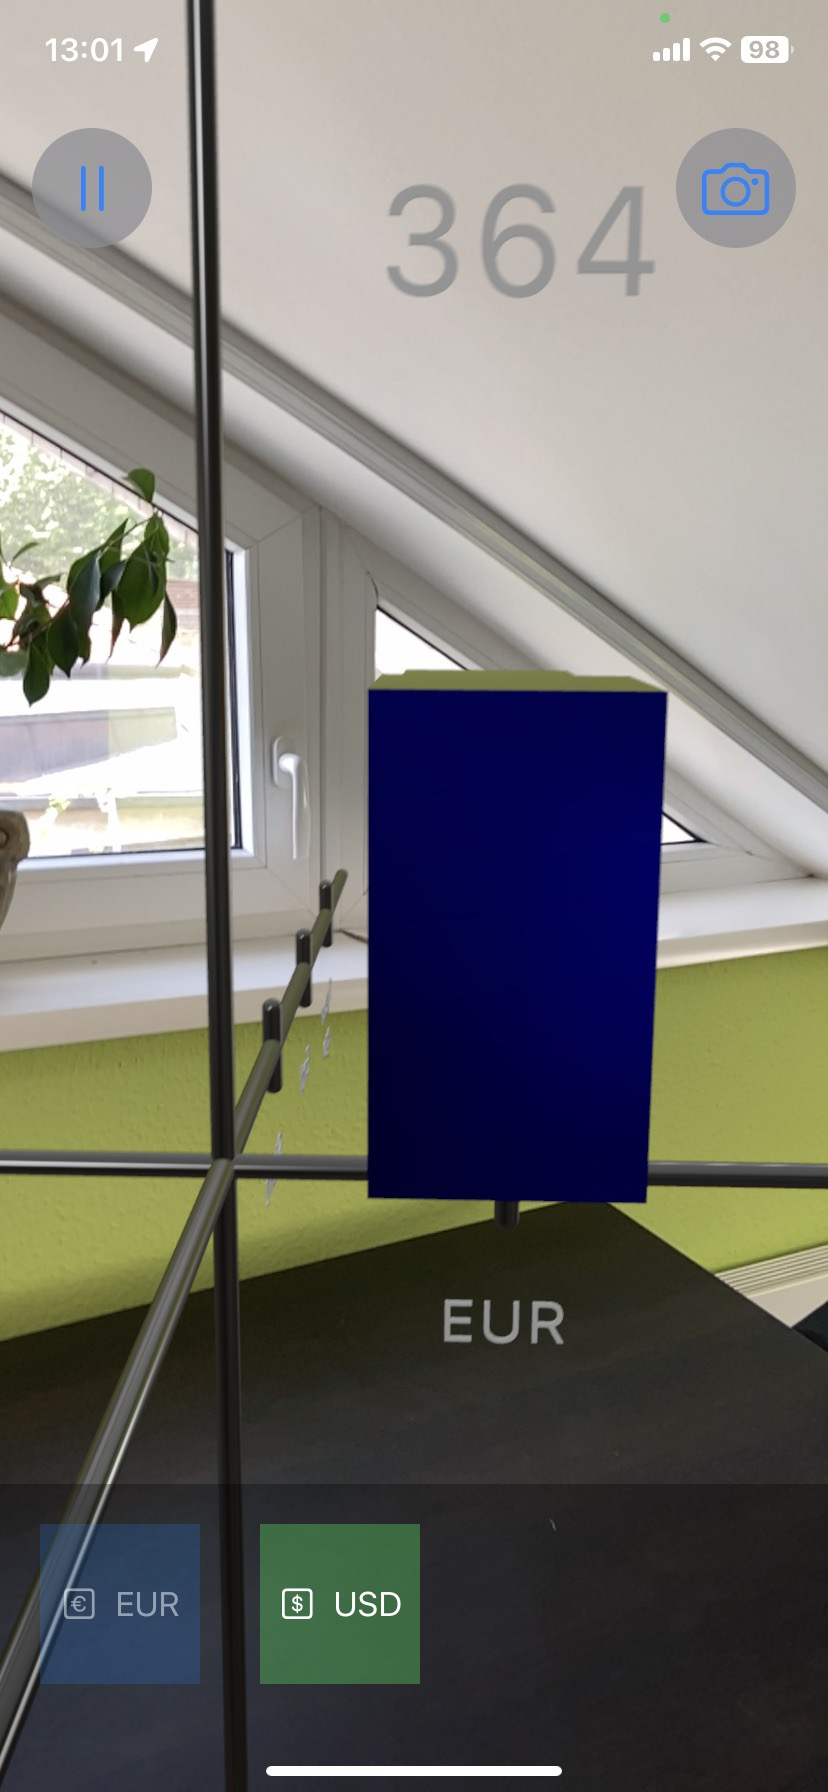
\includegraphics[scale=0.2]{../images/not_available.jpeg}
    % \includegraphics[width=150mm, keepaspectratio]{figures/TeXnicCenter.png}
    \caption{The main screen of the application.}
    \label{fig:TexnicCenter}
\end{figure}
